\documentclass[conference]{IEEEtran}
\usepackage{graphicx}
\usepackage{amsmath}
\usepackage{booktabs}
\usepackage{cite}
\usepackage{url}
\usepackage{xcolor}
\usepackage{balance}

\title{LiDAR-Assisted Reflector Geometry for\\Non-Line-of-Sight Radar Imaging}

\author{\IEEEauthorblockN{Steven Chen}}

\begin{document}
\maketitle

\begin{abstract}
Radar can sense objects hidden around corners by exploiting reflections from visible surfaces, but reconstruction accuracy depends on the geometry assigned to the reflecting surface. We present a LiDAR-assisted pipeline that registers radar and LiDAR measurements, extracts a finite relay surface from the LiDAR point cloud, estimates local surface normals, and relocates indirect radar returns by specular reflection while preserving measured path length. Preliminary experiments cover five target configurations under plain-drywall and foil-covered-wall conditions. Relative to a radar-derived plane, the LiDAR surface reduces median reflector-agreement error from 13.69 to 0.48~cm on drywall and from 6.30 to 0.52~cm with foil. It also reduces mean nearest-target distance from 38.65 to 31.09~cm and from 27.25 to 16.98~cm, respectively. These results support measured reflector geometry as a practical route to more accurate non-line-of-sight localization.
\end{abstract}

\section{Introduction}
Robots and vehicles often must act before a hidden region enters direct view. Radar can probe such regions through a visible wall, but an indirect path places a target return at an apparent ``ghost'' location. Recovering the physical target therefore requires an accurate model of the reflecting surface~\cite{scheiner2020corners,dodds2024rflect,cui2024seeing}.

Prior systems estimate planar or more general reflector geometry from radar measurements~\cite{cui2024seeing,dodds2024rflect}. Sparse radar returns, however, make wall position, orientation, and finite extent difficult to recover. Small geometric errors alter the inferred path and can substantially displace a corrected target. Our project asks whether directly measured LiDAR geometry improves point-level non-line-of-sight (NLOS) radar correction.

We develop a pipeline in which radar supplies the indirect target observations and LiDAR supplies the relay-surface geometry. The contributions at this midterm stage are: (1) a finite, measurement-supported wall model with learned local normals; (2) a path-length-preserving correction that uses ray--surface intersections rather than an infinite plane; and (3) a ten-acquisition comparison against radar-only planar mirroring. We evaluate reflector agreement, target localization, and qualitative target-region completeness. The current evidence is promising but remains an in-sample, single-wall study.

\section{Methods}
\subsection{Measurements and Surface Reconstruction}
All observations are expressed in the LiDAR frame. For apparent radar point $\mathbf{p}_i^R$, radar origin $\mathbf{o}^R$, coordinate map $Q$, and translation $\mathbf{t}$, we compute
\begin{equation}
\mathbf{p}_i=Q\mathbf{p}_i^R+\mathbf{t},\quad
\mathbf{o}=Q\mathbf{o}^R+\mathbf{t},\quad
r_i=\|\mathbf{p}_i-\mathbf{o}\|,
\end{equation}
with scan direction $\mathbf{u}_i=(\mathbf{p}_i-\mathbf{o})/r_i$. The supplied map, including its handedness conversion, is applied consistently to points and the sensor origin.

We predict normals for one LiDAR frame with the released pretrained LiSu model~\cite{malic2025lisu}. Normals are normalized, oriented toward the LiDAR origin, and used with screened Poisson reconstruction~\cite{kazhdan2013screened}. A radar-derived plane seeds wall selection, but the retained reflector is finite: points must be near the seed plane, have compatible normals, and belong to the largest connected region in the organized scan. Triangles are retained only when their vertices and centroid have nearby measured support. This prevents unsupported mesh extensions from acting as reflectors.

\subsection{Local Reflection Correction}
Each distinct radar ray is intersected with the selected mesh. If $s_i$ is the first positive intersection distance, the hit is $\mathbf{h}_i=\mathbf{o}+s_i\mathbf{u}_i$. A local unit normal $\mathbf{n}_i$ is a Gaussian-weighted average of nearby, sign-aligned LiDAR normals. We reject geometry with insufficient neighbors, excessive angular dispersion, disagreement with the intersected face, or an implausible incidence angle.

For accepted geometry, the remaining range is $\ell_i=r_i-s_i$. Returns lying beyond the local tangent plane are candidates for correction; points close to the relay surface remain unchanged. The reflected direction and corrected location are
\begin{equation}
\mathbf{v}_i=\mathbf{u}_i-2(\mathbf{u}_i^T\mathbf{n}_i)\mathbf{n}_i,\qquad
\widehat{\mathbf{x}}_i=\mathbf{h}_i+\ell_i\mathbf{v}_i.
\end{equation}
This construction conserves equivalent one-way path length:
\begin{equation}
\|\mathbf{h}_i-\mathbf{o}\|+\|\widehat{\mathbf{x}}_i-\mathbf{h}_i\|=r_i.
\end{equation}
The implementation saves corrected points, source indices, intersections, normals, and status flags. It uses local geometry within one radar-seeded reflector and does not estimate material reflectivity or arbitrary multi-bounce paths.

\subsection{Experimental Design}
We test five target configurations under two relay conditions: exposed drywall and the same wall covered with reflective foil. The set includes rectangle, L-shape, triangle, mannequin, and triangle--mannequin scenes, for ten acquisitions total. Radar-only planar mirroring is the baseline. The assisted method changes only the relay geometry; radar observations and downstream comparison procedures are otherwise shared.

Reflector agreement is evaluated against selected LiDAR wall samples within 7.5~m of the calibrated radar origin. To separate fit from finite coverage, samples are restricted to each radar plane footprint and voxelized at 5~cm. Target localization uses nearest distance to an independently captured LiDAR target. We also inspect target-region point counts and scene F-score, while treating the latter cautiously because its reference includes visible scene surfaces.

\begin{figure}[t]
  \centering
  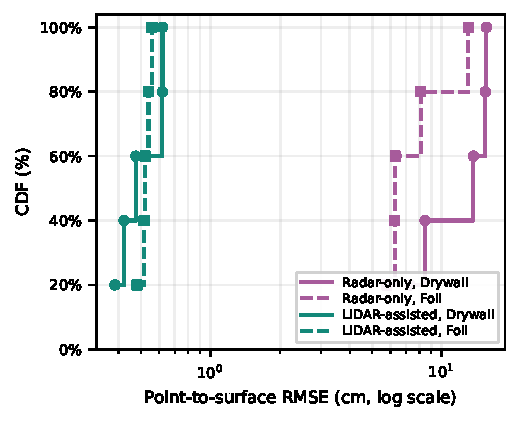
\includegraphics[width=\columnwidth]{figures/wall_surface_cdf_by_reflector.pdf}
  \caption{Reflector-geometry RMSE across five acquisitions per relay condition. The LiDAR-assisted surface agrees more closely with measured wall samples than the radar-only plane. Lower is better.}
  \label{fig:wall}
\end{figure}

\section{Partial Results}
\subsection{Reflector and Target Accuracy}
Figure~\ref{fig:wall} shows a clear separation between geometry methods. On plain drywall, median wall RMSE decreases from 13.69~cm for the radar-only plane to 0.48~cm for the LiDAR-assisted surface. With foil, it decreases from 6.30 to 0.52~cm. Across all acquisitions, assisted RMSE remains below 0.63~cm, whereas planar values range from 5.77 to 15.59~cm. Because the LiDAR measurement constructs and evaluates the surface, this measures internal geometric agreement rather than independent wall accuracy.

Improved geometry also corresponds to better target localization. Mean nearest-target distance falls from 38.65 to 31.09~cm on drywall and from 27.25 to 16.98~cm with foil. These reductions are 7.56~cm (19.6\%) and 10.27~cm (37.7\%), respectively. The larger foil gain is consistent with stronger reflected radar returns, while the drywall result indicates that better geometry remains useful under weaker reflection.

\begin{figure}[t]
  \centering
  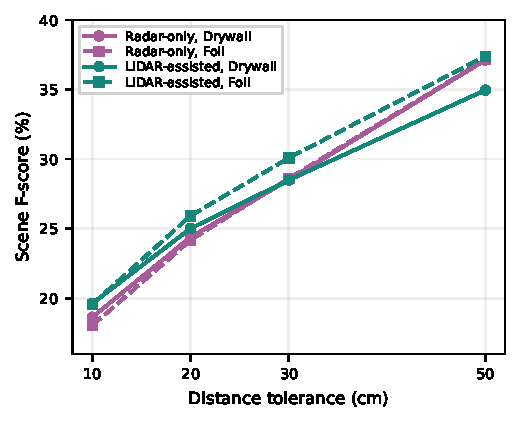
\includegraphics[width=\columnwidth]{figures/whole_scene_fscore_by_reflector.pdf}
  \caption{Mean whole-scene F-score over five target configurations. Assisted correction improves close spatial agreement, especially with foil, but gains are not consistent at broad tolerances. Higher is better.}
  \label{fig:fscore}
\end{figure}

\subsection{Scene Agreement and Completeness}
At a 10~cm tolerance, mean scene F-score rises from 18.64\% to 19.62\% for drywall and from 18.03\% to 19.56\% for foil (Fig.~\ref{fig:fscore}). At 20~cm, gains are 0.63 and 1.75 percentage points, and nine of ten acquisitions improve. The trend weakens at broader tolerances: at 50~cm the changes are $-2.16$ points for drywall and $+0.25$ points for foil. Thus, measured geometry improves close spatial agreement but does not yet guarantee a global scene gain.

The foil reconstructions also retain more target-region returns than planar mirroring: 4,081 versus 3,501 for the rectangle, 4,602 versus 3,542 for the L-shape, 7,552 versus 6,190 for the triangle, and 6,879 versus 4,727 for the triangle--mannequin scene. Figure~\ref{fig:pipeline} compares these reconstructions with the corresponding scene photographs and weak plain-drywall returns. The recovered clusters preserve target-dependent structure, including the rectangle, horizontal L-shape arm, and two components of the combined scene. These counts and views indicate improved completeness, but they are not a shape metric because the region can still include multipath clutter.

\begin{figure*}[t]
  \centering
  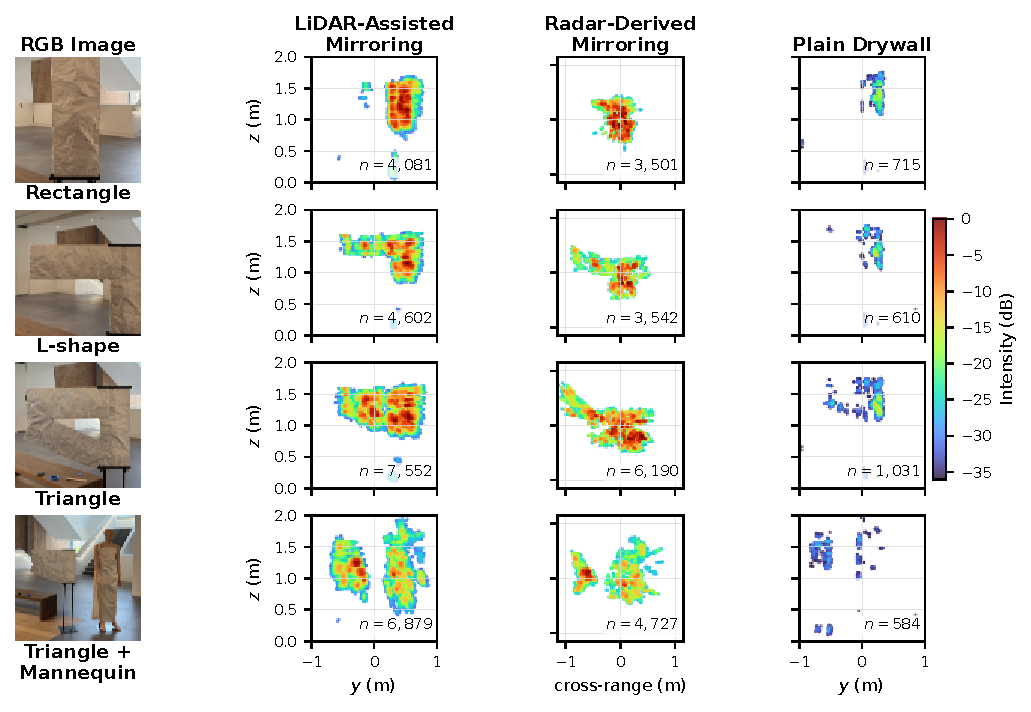
\includegraphics[width=0.92\textwidth]{figures/object_shape_raw_roi.pdf}
  \caption{Target-region radar returns for four scenes. LiDAR-assisted mirroring with foil retains more points and clearer target-dependent structure than radar-derived mirroring; plain drywall produces substantially weaker returns. Color denotes intensity.}
  \label{fig:pipeline}
\end{figure*}

\section{Partial Discussion}
The results support the central hypothesis: measuring the relay surface removes a major source of NLOS correction error. The largest and most consistent improvement is reflector agreement, which is expected because the assisted representation retains wall extent and local orientation. Improvements in nearest-target distance show that this geometric benefit propagates to the hidden region rather than remaining confined to the wall model. The incomplete gains in whole-scene F-score also reveal that reflector geometry is only one error source.

Three limitations shape the next phase. First, the current wall metric is in-sample, and the scene reference includes areas outside effective radar coverage. Second, the target-region analysis uses a manually defined region and point counts rather than registered object-only surfaces. Third, calibration uncertainty, material response, and multiple reflections are not estimated. We will address these limitations with held-out wall measurements, object masks or reference meshes, target-level Chamfer/F-score measures, and sensitivity tests over calibration and surface-selection thresholds. Repeated trials and uncertainty intervals will distinguish stable gains from acquisition-specific effects.

\section{Acknowledgments}
The authors thank the course instructional team for feedback and access to project resources.

\section*{CRediT Author Statement}
Steven Chen: experimental setup, data evaluation, and paper writeup.

\balance
\bibliographystyle{IEEEtran}
\bibliography{references}

\end{document}
